% Options for packages loaded elsewhere
\PassOptionsToPackage{unicode}{hyperref}
\PassOptionsToPackage{hyphens}{url}
%
\documentclass[
  ignorenonframetext,
]{beamer}
\usepackage{pgfpages}
\setbeamertemplate{caption}[numbered]
\setbeamertemplate{caption label separator}{: }
\setbeamercolor{caption name}{fg=normal text.fg}
\beamertemplatenavigationsymbolsempty
% Prevent slide breaks in the middle of a paragraph
\widowpenalties 1 10000
\raggedbottom
\setbeamertemplate{part page}{
  \centering
  \begin{beamercolorbox}[sep=16pt,center]{part title}
    \usebeamerfont{part title}\insertpart\par
  \end{beamercolorbox}
}
\setbeamertemplate{section page}{
  \centering
  \begin{beamercolorbox}[sep=12pt,center]{part title}
    \usebeamerfont{section title}\insertsection\par
  \end{beamercolorbox}
}
\setbeamertemplate{subsection page}{
  \centering
  \begin{beamercolorbox}[sep=8pt,center]{part title}
    \usebeamerfont{subsection title}\insertsubsection\par
  \end{beamercolorbox}
}
\AtBeginPart{
  \frame{\partpage}
}
\AtBeginSection{
  \ifbibliography
  \else
    \frame{\sectionpage}
  \fi
}
\AtBeginSubsection{
  \frame{\subsectionpage}
}
\usepackage{lmodern}
\usepackage{amssymb,amsmath}
\usepackage{ifxetex,ifluatex}
\ifnum 0\ifxetex 1\fi\ifluatex 1\fi=0 % if pdftex
  \usepackage[T1]{fontenc}
  \usepackage[utf8]{inputenc}
  \usepackage{textcomp} % provide euro and other symbols
\else % if luatex or xetex
  \usepackage{unicode-math}
  \defaultfontfeatures{Scale=MatchLowercase}
  \defaultfontfeatures[\rmfamily]{Ligatures=TeX,Scale=1}
\fi
\usetheme[]{Marburg}
\usefonttheme{structurebold}
% Use upquote if available, for straight quotes in verbatim environments
\IfFileExists{upquote.sty}{\usepackage{upquote}}{}
\IfFileExists{microtype.sty}{% use microtype if available
  \usepackage[]{microtype}
  \UseMicrotypeSet[protrusion]{basicmath} % disable protrusion for tt fonts
}{}
\makeatletter
\@ifundefined{KOMAClassName}{% if non-KOMA class
  \IfFileExists{parskip.sty}{%
    \usepackage{parskip}
  }{% else
    \setlength{\parindent}{0pt}
    \setlength{\parskip}{6pt plus 2pt minus 1pt}}
}{% if KOMA class
  \KOMAoptions{parskip=half}}
\makeatother
\usepackage{xcolor}
\IfFileExists{xurl.sty}{\usepackage{xurl}}{} % add URL line breaks if available
\IfFileExists{bookmark.sty}{\usepackage{bookmark}}{\usepackage{hyperref}}
\hypersetup{
  pdftitle={Estadística Inferencial},
  pdfauthor={Jackson M'coy Romero Plasencia},
  hidelinks,
  pdfcreator={LaTeX via pandoc}}
\urlstyle{same} % disable monospaced font for URLs
\newif\ifbibliography
\usepackage{color}
\usepackage{fancyvrb}
\newcommand{\VerbBar}{|}
\newcommand{\VERB}{\Verb[commandchars=\\\{\}]}
\DefineVerbatimEnvironment{Highlighting}{Verbatim}{commandchars=\\\{\}}
% Add ',fontsize=\small' for more characters per line
\usepackage{framed}
\definecolor{shadecolor}{RGB}{248,248,248}
\newenvironment{Shaded}{\begin{snugshade}}{\end{snugshade}}
\newcommand{\AlertTok}[1]{\textcolor[rgb]{0.94,0.16,0.16}{#1}}
\newcommand{\AnnotationTok}[1]{\textcolor[rgb]{0.56,0.35,0.01}{\textbf{\textit{#1}}}}
\newcommand{\AttributeTok}[1]{\textcolor[rgb]{0.77,0.63,0.00}{#1}}
\newcommand{\BaseNTok}[1]{\textcolor[rgb]{0.00,0.00,0.81}{#1}}
\newcommand{\BuiltInTok}[1]{#1}
\newcommand{\CharTok}[1]{\textcolor[rgb]{0.31,0.60,0.02}{#1}}
\newcommand{\CommentTok}[1]{\textcolor[rgb]{0.56,0.35,0.01}{\textit{#1}}}
\newcommand{\CommentVarTok}[1]{\textcolor[rgb]{0.56,0.35,0.01}{\textbf{\textit{#1}}}}
\newcommand{\ConstantTok}[1]{\textcolor[rgb]{0.00,0.00,0.00}{#1}}
\newcommand{\ControlFlowTok}[1]{\textcolor[rgb]{0.13,0.29,0.53}{\textbf{#1}}}
\newcommand{\DataTypeTok}[1]{\textcolor[rgb]{0.13,0.29,0.53}{#1}}
\newcommand{\DecValTok}[1]{\textcolor[rgb]{0.00,0.00,0.81}{#1}}
\newcommand{\DocumentationTok}[1]{\textcolor[rgb]{0.56,0.35,0.01}{\textbf{\textit{#1}}}}
\newcommand{\ErrorTok}[1]{\textcolor[rgb]{0.64,0.00,0.00}{\textbf{#1}}}
\newcommand{\ExtensionTok}[1]{#1}
\newcommand{\FloatTok}[1]{\textcolor[rgb]{0.00,0.00,0.81}{#1}}
\newcommand{\FunctionTok}[1]{\textcolor[rgb]{0.00,0.00,0.00}{#1}}
\newcommand{\ImportTok}[1]{#1}
\newcommand{\InformationTok}[1]{\textcolor[rgb]{0.56,0.35,0.01}{\textbf{\textit{#1}}}}
\newcommand{\KeywordTok}[1]{\textcolor[rgb]{0.13,0.29,0.53}{\textbf{#1}}}
\newcommand{\NormalTok}[1]{#1}
\newcommand{\OperatorTok}[1]{\textcolor[rgb]{0.81,0.36,0.00}{\textbf{#1}}}
\newcommand{\OtherTok}[1]{\textcolor[rgb]{0.56,0.35,0.01}{#1}}
\newcommand{\PreprocessorTok}[1]{\textcolor[rgb]{0.56,0.35,0.01}{\textit{#1}}}
\newcommand{\RegionMarkerTok}[1]{#1}
\newcommand{\SpecialCharTok}[1]{\textcolor[rgb]{0.00,0.00,0.00}{#1}}
\newcommand{\SpecialStringTok}[1]{\textcolor[rgb]{0.31,0.60,0.02}{#1}}
\newcommand{\StringTok}[1]{\textcolor[rgb]{0.31,0.60,0.02}{#1}}
\newcommand{\VariableTok}[1]{\textcolor[rgb]{0.00,0.00,0.00}{#1}}
\newcommand{\VerbatimStringTok}[1]{\textcolor[rgb]{0.31,0.60,0.02}{#1}}
\newcommand{\WarningTok}[1]{\textcolor[rgb]{0.56,0.35,0.01}{\textbf{\textit{#1}}}}
\usepackage{graphicx,grffile}
\makeatletter
\def\maxwidth{\ifdim\Gin@nat@width>\linewidth\linewidth\else\Gin@nat@width\fi}
\def\maxheight{\ifdim\Gin@nat@height>\textheight\textheight\else\Gin@nat@height\fi}
\makeatother
% Scale images if necessary, so that they will not overflow the page
% margins by default, and it is still possible to overwrite the defaults
% using explicit options in \includegraphics[width, height, ...]{}
\setkeys{Gin}{width=\maxwidth,height=\maxheight,keepaspectratio}
% Set default figure placement to htbp
\makeatletter
\def\fps@figure{htbp}
\makeatother
\setlength{\emergencystretch}{3em} % prevent overfull lines
\providecommand{\tightlist}{%
  \setlength{\itemsep}{0pt}\setlength{\parskip}{0pt}}
\setcounter{secnumdepth}{-\maxdimen} % remove section numbering
\usepackage{ragged2e}
\usepackage{color}
\usepackage{listings}
\usepackage{multicol}
\AtBeginSubsection{}

\title{Estadística Inferencial}
\author{Jackson M'coy Romero Plasencia}
\date{Ayacucho 2020}
\institute{\large Universidad Nacional de San Cristóbal de Huamanga \and \normalsize Departamento Académico de Matemática y Física}

\begin{document}
\frame{\titlepage}

\begin{frame}
  \tableofcontents[hideallsubsections]
\end{frame}
\hypertarget{retroalimentaciuxf3n}{%
\section{Retroalimentación}\label{retroalimentaciuxf3n}}

\hypertarget{definiciuxf3n-muestra-aleatoria}{%
\subsection{Definición: Muestra
Aleatoria}\label{definiciuxf3n-muestra-aleatoria}}

\begin{frame}{Definición: Muestra Aleatoria}

Una muestra aleatoria de tamaño \(n\) de una variable aleatorio \(X\) es
un conjunto de \(n\) - variables aleatorias \(X_1,X_2,...,X_n\), tal
que:

\begin{itemize}
  \item Todas $X_1,X_2,...,X_n \quad i=\overline{1,n}$ son independientes
  \item $X_1,X_2,...,X_n$ tienen la misma distribución, es decir:
        $$F_{X_i}(t)=F_{X}(t)\quad \forall \,\,i=\overline{1,n}$$
        $$\quad \longrightarrow f_{X_1,X_2,...,X_n}(x_1,x_2,...,x_n)=\prod_{i=1}^{n} f_{X_i}(x_i) $$
\end{itemize}

\end{frame}

\hypertarget{section}{%
\subsection{}\label{section}}

\begin{frame}{}

Ejercicio propuesto:

Si \(X\) es una variable aleatoria, con:
\[f_X(x,p)=f_X (x)= p^x (1-p)^{1-x},\quad x=0,1 \quad 0<p<1\] y sea una
muestra aleatoria de tamaño \(n\) . Hállese la distribución.

\[Y=\displaystyle \sum_{i=1}^{n}X_i\]

Función Generatriz de Momentos: \(M_X(t)\)

\[fgm(x)=M_X (t)=\mathbb{E}[e^{tx}] \] Primero se determinará la
\(M_X(t)\) en la población

\end{frame}

\hypertarget{section-1}{%
\subsection{}\label{section-1}}

\begin{frame}{}

\[f_X(x,p)=f_X (x)= p^x (1-p)^{1-x},\quad x=0,1 \quad 0<p<1\]
\[\begin{matrix}
M_X(t) & = & \mathbb{E}[e^{tx}] & = &\displaystyle\sum_{x=0}^{1} \,e^{tx} \,p^x \,(1-p)^{1-x} \\ 
 &  &  &=  & \displaystyle\sum_{x=0}^{1} \,(pe^t)^{x} \,(1-p)^{1-x}\\
 &  &  &=  &  ((1-p)+pe^t)
\end{matrix}
\]

\justifying Primera forma: Usando la Función de Generatriz de Momentos:
\(Y=\displaystyle \sum_{i=1}^{n}X_i\)

\[\begin{matrix}
M_Y(t) & = & \mathbb{E}[e^{ty}] & = & \mathbb{E}[e^{t(X_1+X_2+...+X_n)}] \\  &  &  &=  & \mathbb{E}[e^{t(X_1)} \, e^{t(X_2)}...e^{t(X_n)}] \\
 &  &  &=  & \mathbb{E}[e^{t(X_1)}] \, \mathbb{E}[e^{t(X_2)}]... \,\mathbb{E}[e^{t(X_n)}]\\
 &  &  &=  &\big(\mathbb{E}[e^{t(X_i)}]\big)^n\\
  &  &  &=  &\bigg((1-p)+pe^t\bigg)^n \longrightarrow Bin(n,p)
\end{matrix}
\]

\end{frame}

\hypertarget{section-2}{%
\subsection{}\label{section-2}}

\begin{frame}{}

Segunda forma:
\[f_X(x,n,p)=f_X (x)= \binom{n}{p} p^x (1-p)^{1-x},\quad x=\overline{0,n} \quad 0<p<1\]
Es la función de probabilidad de la Distribución Binomial.

\[\mathbb{E}(X)=np \quad \mbox{y}\quad \mathbb{V}(X)=npq \]
\[\begin{matrix}
\mathbb{E}(Y) & = & \mathbb{E}(X_1+X_2+...+
X_n) & = & \mathbb{E}(X_1)+...+\mathbb{E}(X_n)\\ 
 &  &  &=  &\underbrace{p+p+...+p}_{n \,\,veces} =np\\
\mathbb{V}(Y) & = & \mathbb{V}(X_1+X_2+...+
X_n) & = & \mathbb{V}(X_1)+...+\mathbb{V}(X_n)\\ 
 &  &  &=  &\underbrace{pq+pq+...+pq}_{n \,\,veces} =npq
\end{matrix}
\]

\end{frame}

\hypertarget{distribuciuxf3n-de-la-media-muestral}{%
\section{Distribución de la Media
Muestral}\label{distribuciuxf3n-de-la-media-muestral}}

\hypertarget{distribuciuxf3n-de-la-media-muestral-1}{%
\subsection{Distribución de la Media
Muestral}\label{distribuciuxf3n-de-la-media-muestral-1}}

\begin{frame}{Distribución de la Media Muestral}

\justifying Si \(X_1,X_2,...,X_n\) es unas muestra aleatoria de una
población infinita, con media \(\mu\) y varianza \(\sigma^2<\infty\),
entonces:

\[\mathbb{E}(\overline{X} )=\mu \quad\quad \mathbb{V}(\overline{X} )=\frac{\sigma^2}{n} \]
Demostración:

Como \(\overline{X}=\displaystyle \sum_{i=1}^{n}\frac{X_i}{n}\),
entonces:

\[\mathbb{E}(\overline{X} )  = \mathbb{E}\bigg(\displaystyle\sum_{i=1}^{n}\frac{X_i}{n} \bigg )=\displaystyle \sum_{i=1}^{n}\frac{\mathbb{E} (X_i)}{n}= \displaystyle \sum_{i=1}^{n}\frac{\mu}{n}= \mu\]
\[\mathbb{V}(\overline{X} )= \mathbb{V}\bigg(\displaystyle \sum_{i=1}^{n}\frac{X_i}{n} \bigg) = \displaystyle \sum_{i=1}^{n}\frac{\mathbb{V} (X_i)}{n^2}  = \displaystyle \sum_{i=1}^{n}\frac{\sigma^2}{n^2}=\displaystyle\frac{\sigma^2}{n}\]

Por consiguiente:
\(\overline{X} \longrightarrow N(\mu, \displaystyle \frac{\sigma^2}{n})\)

\end{frame}

\hypertarget{section-3}{%
\subsection{}\label{section-3}}

\begin{frame}{}

Ejemplo: \justifying Una fábrica textil tiene 5 operarios. Los años de
servicio en la fábrica de estos operarios son: \[3,4,7,9,12\]

\begin{itemize}
\justifying
  \item [a.] Calcule la media y varianza de la población
  \item [b.] Determine la distribución de la media de las muestras de tamaño 2 de la población(reposición)
  \item [c.] Determine la distribución de la media de las muestras de tamaño 2 de la población(sin reposición)
  
\end{itemize}

Solución:

\begin{enumerate}
[a.]
\tightlist
\item
  Media y varianza de la población
\end{enumerate}

\[\mathbb{E}(X)=\sum_{i=1}^{n} x_if(x_i) \quad\mbox{y} \quad \mathbb{V}(X)= \mathbb{E}(X^2)-(\mathbb{E}(X))^2\]

\[\mathbb{E}(X)=\sum_{i=1}^{n} x_if(x_i)=3(1/5)+4(1/5)+...+12(1/5)=7\]

\end{frame}

\hypertarget{section-4}{%
\subsection{}\label{section-4}}

\begin{frame}[fragile]{}

\[\mathbb{E}(X^2)=\sum_{i=1}^{n} x_i^2f(x_i)=3^2(1/5)+4^2(1/5)+...+12^2(1/5)=59.8\]
\(\mathbb{V}(X)= \mathbb{E}(X^2)-(\mathbb{E}(X))^2=59.8-7^2=10.8\)

luego:
\[\mathbb{E}(X)=\mu=7 \quad\quad \mbox{y} \quad\quad  \mathbb{V}(X)=\sigma^2=10.8 \]
En R:

\begin{Shaded}
\begin{Highlighting}[]
\NormalTok{pob<-}\KeywordTok{c}\NormalTok{(}\DecValTok{3}\NormalTok{,}\DecValTok{4}\NormalTok{,}\DecValTok{7}\NormalTok{,}\DecValTok{9}\NormalTok{,}\DecValTok{12}\NormalTok{)}
\KeywordTok{mean}\NormalTok{(pob)}
\end{Highlighting}
\end{Shaded}

\begin{verbatim}
## [1] 7
\end{verbatim}

\begin{Shaded}
\begin{Highlighting}[]
\KeywordTok{var}\NormalTok{(pob) }\CommentTok{#varianza con denominador n-1}
\end{Highlighting}
\end{Shaded}

\begin{verbatim}
## [1] 13.5
\end{verbatim}

\begin{Shaded}
\begin{Highlighting}[]
\KeywordTok{var}\NormalTok{(pob)}\OperatorTok{*}\DecValTok{4}\OperatorTok{/}\DecValTok{5} \CommentTok{#barianza con denomiador n}
\end{Highlighting}
\end{Shaded}

\begin{verbatim}
## [1] 10.8
\end{verbatim}

\end{frame}

\hypertarget{section-5}{%
\subsection{}\label{section-5}}

\begin{frame}{}

\begin{enumerate}
[a.]
\setcounter{enumi}{1}
\tightlist
\item
  Muestras de tamaño 2, con reposición
\end{enumerate}

\begin{multicols}{2}

\begin{center}
\begin{tabular}{ c c c c c}
 3,3 & 3,4 & 3,7 & 3,9 & 3,12\\ 
 4,3 & 4,4 & 4,7 & 4,9 & 4,12\\
 7,3 & 7,4 & 7,7 & 7,9 & 7,12\\
 9,3 & 9,4 & 9,7 & 9,9 & 9,12\\
 3,3 & 3,4 & 3,7 & 3,9 & 12,12
\end{tabular}
\end{center}

\columnbreak

\begin{center}
\begin{tabular}{ c c c c c}
  3.0 & 3.5 & 5.0 & 6.0 & 7.5\\ 
 3.5 & 4.0 & 5.5 & 6.5 & 8.0\\
 5.0 & 5.5 & 7.0 & 8.0 & 9.5\\ 
 6.0 & 6.5 & 8.0 & 9.0 & 10.5\\ 
7.5  & 8.0 &9.5& 10.5 &12.0
\end{tabular}
\end{center}
\end{multicols}

\[\mathbb{E}(\overline{X})=\sum_{i=1}^{n} \overline{x}f(\overline{x}) \quad\mbox{y} \quad \mathbb{V}(\overline{X})= \mathbb{E}(\overline{X}^2)-(\mathbb{E}(\overline{X}))^2\]

\[\mathbb{E}(\overline{X})=\sum_{i=1}^{n} \overline{x}f(\overline{x})=3(1/25)+3.5(2/25)+....+12(1/25)=7 \]

\end{frame}

\hypertarget{section-6}{%
\subsection{}\label{section-6}}

\begin{frame}[fragile]{}

\[\mathbb{E}(\overline{X}^2)=\sum_{i=1}^{n} \overline{x}^2f(\overline{x})=3^2(1/25)+....+12^2(1/25)=\frac{1360}{25} \]

\[\mathbb{V}(\overline{X})= \mathbb{E}(\overline{X}^2)-(\mathbb{E}(\overline{X}))^2=\frac{1360}{25}-7^2 =5.4\]
Se debe tener en cuenta, que:
\(\displaystyle \mathbb{V}(\overline{X})=\sigma_{\overline{x}}^{2}=\frac{\sigma^2}{n}=\frac{10.8}{2}=5.4\)

En R:

\begin{Shaded}
\begin{Highlighting}[]
\NormalTok{pob<-}\KeywordTok{c}\NormalTok{(}\DecValTok{3}\NormalTok{,}\DecValTok{4}\NormalTok{,}\DecValTok{7}\NormalTok{,}\DecValTok{9}\NormalTok{,}\DecValTok{12}\NormalTok{)}
\NormalTok{a<-}\KeywordTok{sapply}\NormalTok{(}\DecValTok{1}\OperatorTok{:}\FloatTok{1e4}\NormalTok{,}\ControlFlowTok{function}\NormalTok{(x)\{}\KeywordTok{mean}\NormalTok{(}\KeywordTok{sample}\NormalTok{(pob,}\DecValTok{2}\NormalTok{,T))\})}
\KeywordTok{mean}\NormalTok{(a)}
\end{Highlighting}
\end{Shaded}

\begin{verbatim}
## [1] 6.9692
\end{verbatim}

\begin{Shaded}
\begin{Highlighting}[]
\KeywordTok{var}\NormalTok{(a)}
\end{Highlighting}
\end{Shaded}

\begin{verbatim}
## [1] 5.335535
\end{verbatim}

\end{frame}

\hypertarget{section-7}{%
\subsection{}\label{section-7}}

\begin{frame}{}

\begin{enumerate}
[a.]
\setcounter{enumi}{2}
\tightlist
\item
  Muestras de tamaño 2, sin reposición
\end{enumerate}

\begin{multicols}{2}

\begin{center}
\begin{tabular}{ c c c c }
  3,4 & 3,7 & 3,9 & 3,12\\ 
 4,3  & 4,7 & 4,9 & 4,12\\
 7,3 & 7,4   & 7,9 & 7,12\\
 9,3 & 9,4 & 9,7   & 9,12\\
 3,3 & 3,4 & 3,7 & 3,9
\end{tabular}
\end{center}

\columnbreak

\begin{center}
\begin{tabular}{ c c c c}
    3.5 & 5.0 & 6.0 & 7.5\\ 
 3.5   & 5.5 & 6.5 & 8.0\\
 5.0 & 5.5   & 8.0 & 9.5\\ 
 6.0 & 6.5 & 8.0   & 10.5\\ 
7.5  & 8.0 &9.5& 10.5 
\end{tabular}
\end{center}
\end{multicols}

\[\mathbb{E}(\overline{X})=\sum_{i=1}^{n} \overline{x}f(\overline{x}) \quad\mbox{y} \quad \mathbb{V}(\overline{X})= \mathbb{E}(\overline{X}^2)-(\mathbb{E}(\overline{X}))^2\]

\[\mathbb{E}(\overline{X})=\sum_{i=1}^{n} \overline{x}f(\overline{x})=3.5(2/20)+5(2/20)+....+10.5(2/20)=7 \]

\end{frame}

\hypertarget{section-8}{%
\subsection{}\label{section-8}}

\begin{frame}[fragile]{}

\[\mathbb{E}(\overline{X}^2)=\sum_{i=1}^{n} \overline{x}^2f(\overline{x})=3.5^2(2/20)+....+10.5^2(2/20)=\frac{1061}{20} \]

\[\mathbb{V}(\overline{X})= \mathbb{E}(\overline{X}^2)-(\mathbb{E}(\overline{X}))^2=\frac{1061}{20}-7^2 =4.05\]
Se debe tener en cuenta, que:
\(\displaystyle \mathbb{V}(\overline{X})=\sigma_{\overline{x}}^{2}=\frac{\sigma^2}{n}\Bigg(\frac{N-n}{N-1}\Bigg) =\frac{10.8}{2}\Bigg(\frac{5-2}{5-1}\Bigg)=4.05\)

En R:

\begin{Shaded}
\begin{Highlighting}[]
\NormalTok{pob<-}\KeywordTok{c}\NormalTok{(}\DecValTok{3}\NormalTok{,}\DecValTok{4}\NormalTok{,}\DecValTok{7}\NormalTok{,}\DecValTok{9}\NormalTok{,}\DecValTok{12}\NormalTok{)}
\NormalTok{a<-}\KeywordTok{replicate}\NormalTok{(}\FloatTok{1e5}\NormalTok{, }\KeywordTok{mean}\NormalTok{(}\KeywordTok{sample}\NormalTok{(pob,}\DecValTok{2}\NormalTok{,F)) )}
\KeywordTok{mean}\NormalTok{(a)}
\end{Highlighting}
\end{Shaded}

\begin{verbatim}
## [1] 6.99492
\end{verbatim}

\begin{Shaded}
\begin{Highlighting}[]
\KeywordTok{var}\NormalTok{(a)}
\end{Highlighting}
\end{Shaded}

\begin{verbatim}
## [1] 4.044285
\end{verbatim}

\end{frame}

\hypertarget{notas}{%
\subsection{Notas}\label{notas}}

\begin{frame}{Notas}

\begin{enumerate}
\justifying

  \item La aproximación de $\overline{X}$ a la distribución normal$(N(\mu, \sigma^2/n))$ es buena, si $n\geq 30$, sin importa si la distribución en discreta o continua.
  \item Si la muestra aleatoria es escogida de una población normal $N(\mu, \sigma^2)$, entonces, la distribución de $\overline{X}$ es exactamente normal $N(\mu, \sigma^2/n)$, para cualquier tamaño de muestra $n \geq 2$
  \item Si el muestro es sin reeemplazo en una población finita de tamaño N, entonces, la varianza de la media muestral es:
    $$ \displaystyle \mathbb{V}(\overline{X})=\sigma_{\overline{x}}^{2}=\frac{\sigma^2}{n}\Bigg(\frac{N-n}{N-1}\Bigg)$$
  El coeficiente $\Bigg(\frac{N-n}{N-1}\Bigg)$ se denomina factor de correción para población finita
  \item La desviación estándar de una estadística es conocidad como error típico o error estándar
\end{enumerate}

\end{frame}

\hypertarget{section-9}{%
\subsection{}\label{section-9}}

\begin{frame}[fragile]{}

\justifying

Ejemplo: El número de automóviles por familia es una variable aleatoria
\(X\) cuya distribución de probabilidad es como sigue:

\begin{center}
\begin{tabular}{ |c |c |c |c |c| c|}
\hline
 $x$  & 0 & 1 & 2 &3 & 4\\ \hline
$f_X(x)$ & 4/12  & 4/12 & 2/12 & 1/11& 1/12 \\ \hline

 \end{tabular}
\end{center}

\begin{itemize}\justifying
  \item  Halle la media y la varianza de la población del número de automóviles por familia.Si se escoge una muestra de 49 familias. ¿Cuál es la probabilidad de que la media muestral de autos por familia esté entre 1 y 2?
\end{itemize}

En R:

\begin{Shaded}
\begin{Highlighting}[]
\CommentTok{#a.}
\NormalTok{poba<-}\KeywordTok{c}\NormalTok{(}\DecValTok{0}\NormalTok{,}\DecValTok{0}\NormalTok{,}\DecValTok{0}\NormalTok{,}\DecValTok{0}\NormalTok{,}\DecValTok{1}\NormalTok{,}\DecValTok{1}\NormalTok{,}\DecValTok{1}\NormalTok{,}\DecValTok{1}\NormalTok{,}\DecValTok{2}\NormalTok{,}\DecValTok{2}\NormalTok{,}\DecValTok{3}\NormalTok{,}\DecValTok{4}\NormalTok{)}
\KeywordTok{mean}\NormalTok{(poba)}
\end{Highlighting}
\end{Shaded}

\begin{verbatim}
## [1] 1.25
\end{verbatim}

\begin{Shaded}
\begin{Highlighting}[]
\KeywordTok{var}\NormalTok{(poba)}\OperatorTok{*}\NormalTok{(}\DecValTok{48}\OperatorTok{/}\DecValTok{49}\NormalTok{)}
\end{Highlighting}
\end{Shaded}

\begin{verbatim}
## [1] 1.625232
\end{verbatim}

\end{frame}

\hypertarget{section-10}{%
\subsection{}\label{section-10}}

\begin{frame}[fragile]{}

\begin{Shaded}
\begin{Highlighting}[]
\CommentTok{#b.}
\NormalTok{poba<-}\KeywordTok{c}\NormalTok{(}\DecValTok{0}\NormalTok{,}\DecValTok{0}\NormalTok{,}\DecValTok{0}\NormalTok{,}\DecValTok{0}\NormalTok{,}\DecValTok{1}\NormalTok{,}\DecValTok{1}\NormalTok{,}\DecValTok{1}\NormalTok{,}\DecValTok{1}\NormalTok{,}\DecValTok{2}\NormalTok{,}\DecValTok{2}\NormalTok{,}\DecValTok{3}\NormalTok{,}\DecValTok{4}\NormalTok{)}
\NormalTok{mues<-}\KeywordTok{sapply}\NormalTok{(}\DecValTok{1}\OperatorTok{:}\FloatTok{1e4}\NormalTok{, }\ControlFlowTok{function}\NormalTok{(x) \{}
\KeywordTok{mean}\NormalTok{(}\KeywordTok{sample}\NormalTok{(poba,}\DecValTok{49}\NormalTok{,T))\} )}
\KeywordTok{mean}\NormalTok{(mues)}
\end{Highlighting}
\end{Shaded}

\begin{verbatim}
## [1] 1.248696
\end{verbatim}

\begin{Shaded}
\begin{Highlighting}[]
\KeywordTok{var}\NormalTok{(mues)}
\end{Highlighting}
\end{Shaded}

\begin{verbatim}
## [1] 0.03100554
\end{verbatim}

\end{frame}

\hypertarget{teorema-central-del-luxedmite}{%
\section{Teorema Central del
Límite}\label{teorema-central-del-luxedmite}}

\hypertarget{desigualdad-de-chebyshev}{%
\subsection{Desigualdad de Chebyshev}\label{desigualdad-de-chebyshev}}

\begin{frame}{Desigualdad de Chebyshev}

\justifying

Sea \(X\) una variablea aleatoria, con media \(\mathbb{E}(X)=\mu\) y
varianza \(\mathbb{V}(X)=\sigma^2\), entonces:

\[\forall \, e>0,\displaystyle  P(|X-\mu|\geq e)\leq \frac{\sigma^2}{e^2}\]

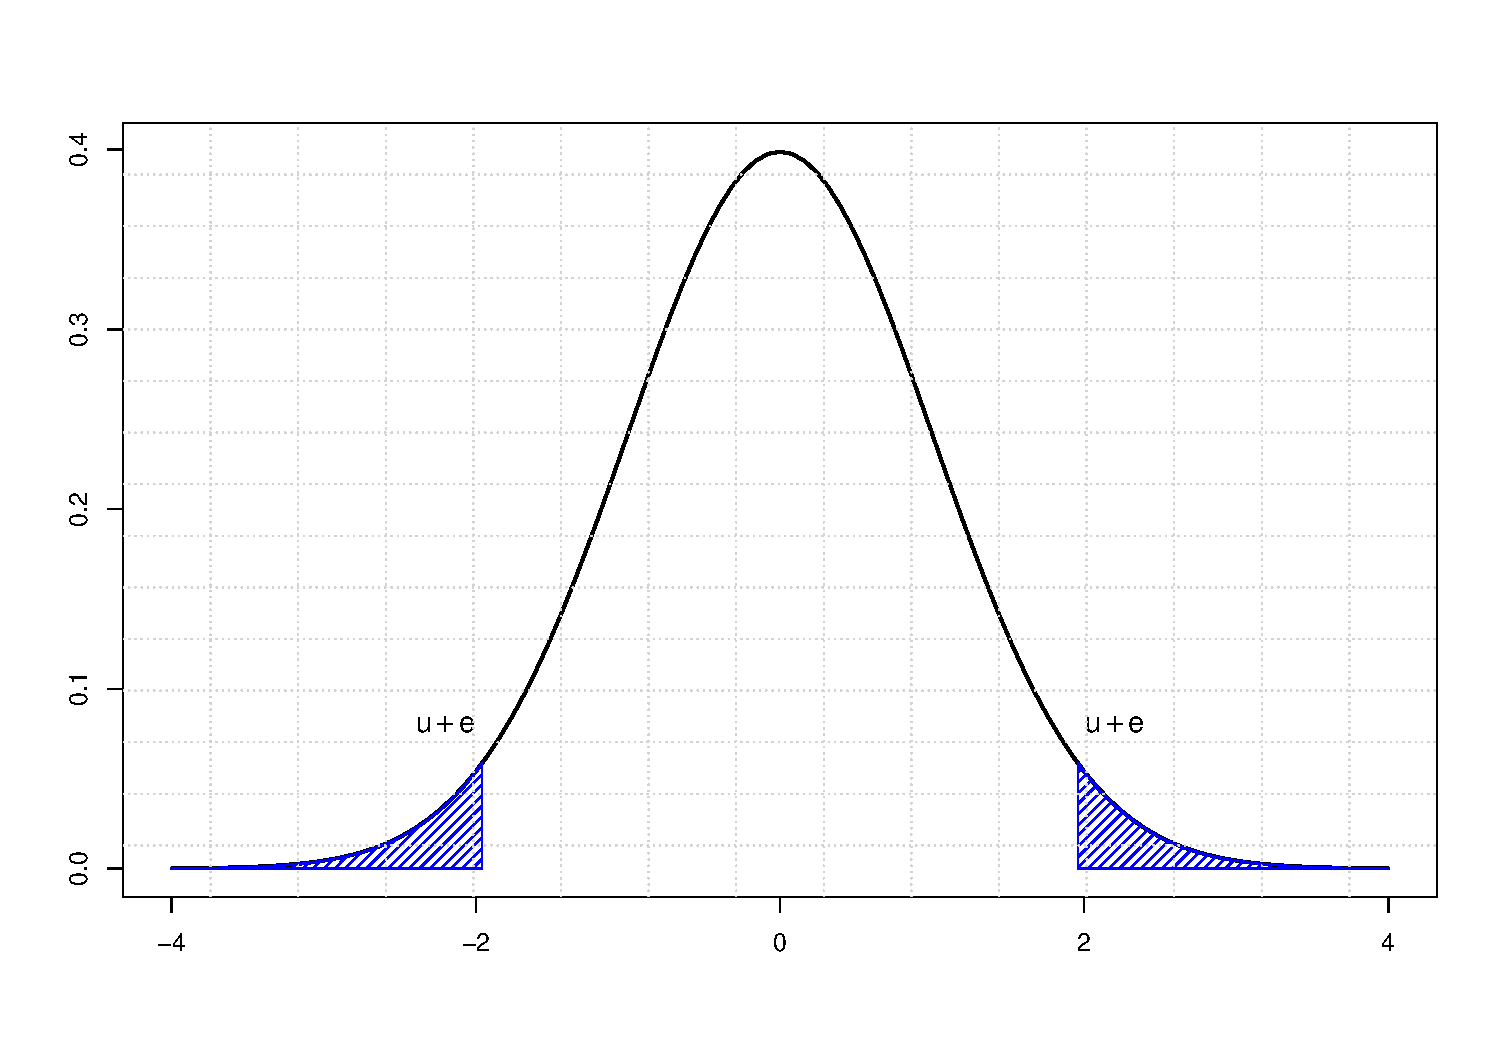
\includegraphics{clase2Inferencia_files/figure-beamer/unnamed-chunk-6-1.pdf}

\end{frame}

\hypertarget{otras-formas-de-la-desigualdad-de-chebyshev}{%
\subsection{Otras formas de la desigualdad de
Chebyshev}\label{otras-formas-de-la-desigualdad-de-chebyshev}}

\begin{frame}[fragile]{Otras formas de la desigualdad de Chebyshev}

\begin{itemize}

\item $\forall \, e>0,\displaystyle  P(|X-\mathbb{E}(X) |\geq e)\leq \frac{\mathbb{V}(X) }{e^2}$
\item $\forall \, k\geq 1,\displaystyle  P(|X-\mu|\geq k\,\sigma)\leq \frac{1}{k^2}$
\end{itemize}

Ejemplo: Sea \(X\) una variable aleatorio con distribución normal
estándar \(N(0,1)\). Hallar el valor de: \(P(-2\leq X \leq 2)\)

\begin{center}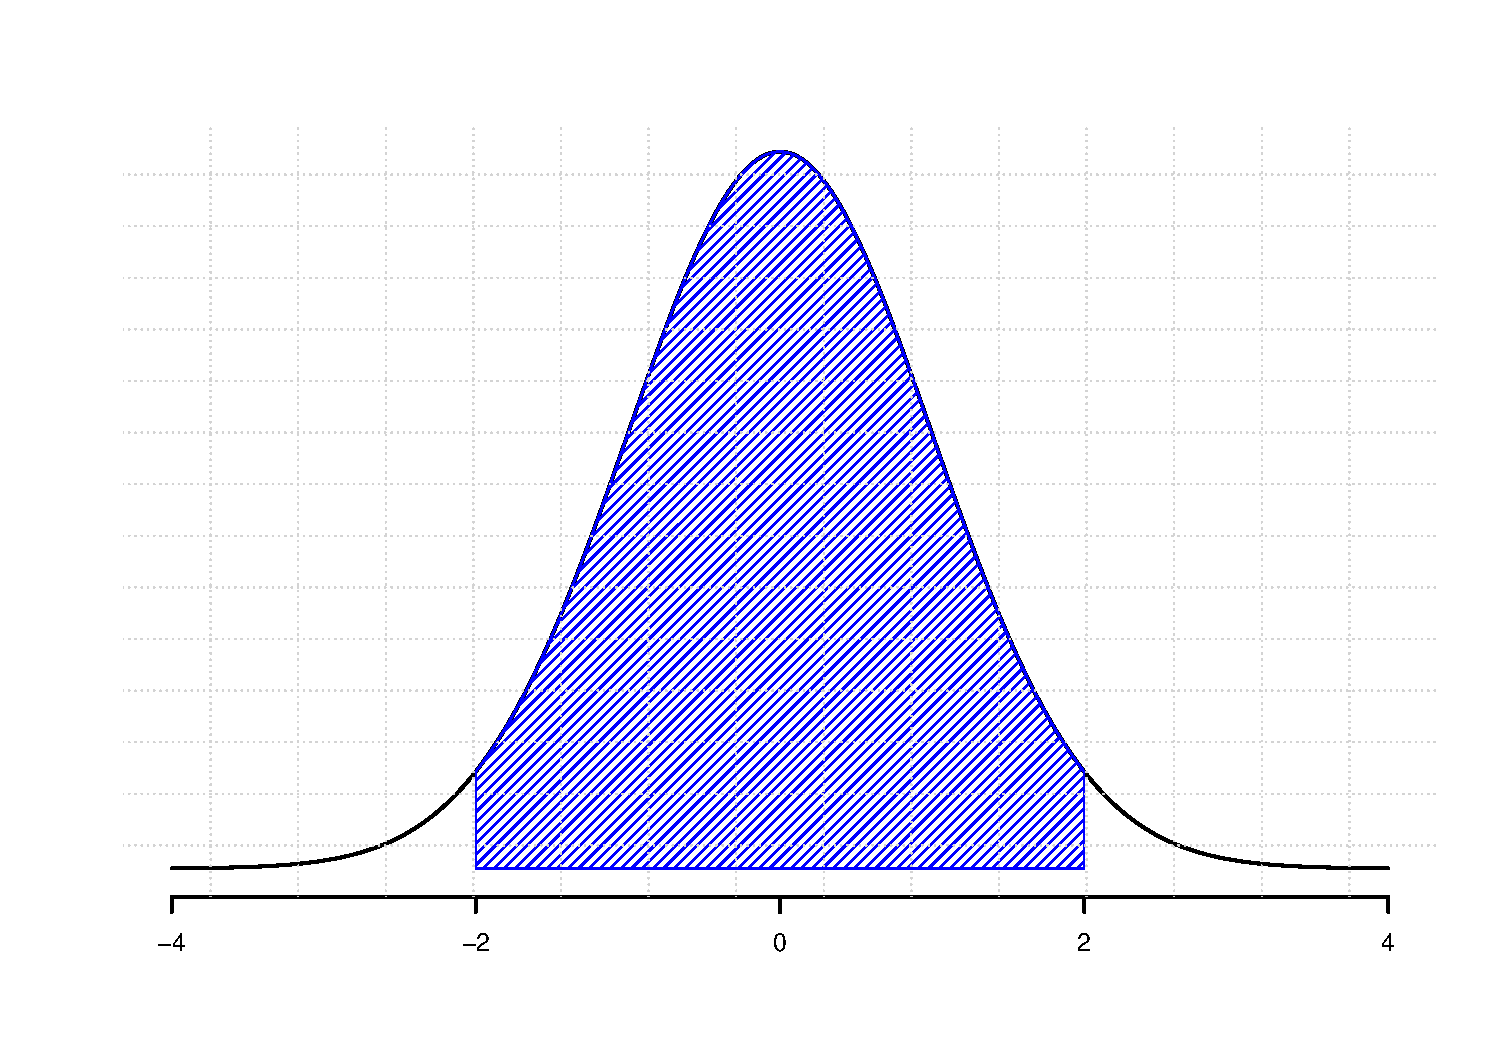
\includegraphics[width=0.4\linewidth]{clase2Inferencia_files/figure-beamer/unnamed-chunk-7-1} \end{center}

\begin{Shaded}
\begin{Highlighting}[]
\KeywordTok{pnorm}\NormalTok{(}\DecValTok{2}\NormalTok{)}\OperatorTok{-}\KeywordTok{pnorm}\NormalTok{(}\OperatorTok{-}\DecValTok{2}\NormalTok{)}
\end{Highlighting}
\end{Shaded}

\begin{verbatim}
## [1] 0.9544997
\end{verbatim}

\end{frame}

\hypertarget{ley-de-los-grandes-nuxfameros}{%
\subsection{Ley de los grandes
números}\label{ley-de-los-grandes-nuxfameros}}

\begin{frame}{Ley de los grandes números}

\justifying Sea \(\{X_n\}_{n\in N}\) una sucesión de variables
aleatorias independientes e indénticamente distribuídas con media
\(\mu < \infty\). Entonces:
\[\displaystyle \frac{1}{n} \sum_{i=1}^{n}X_i  \xrightarrow[n\rightarrow{}\infty]\,{\mu}\]
en donde la convergencia se cumple en el sentido casi seguro(ley fuerte)
y también en probabilidad (ley débil) Seam \(X1_,X_2,...\) v.a con
distribución de \(Bernoulli(p=0.5)\)

\begin{center}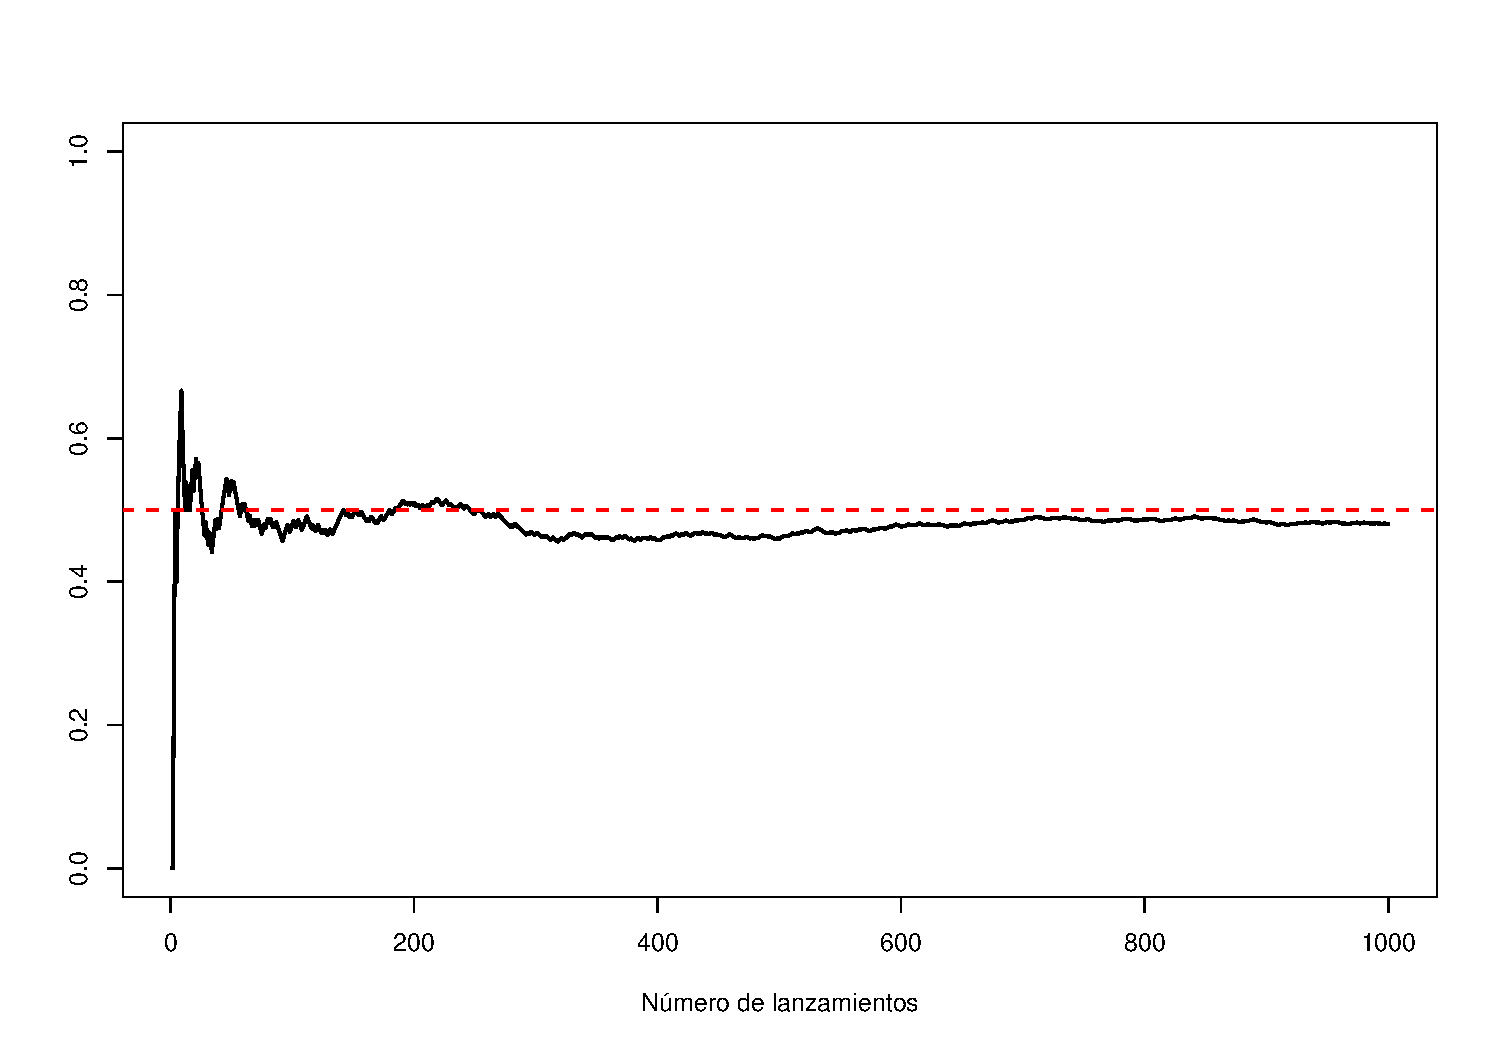
\includegraphics[width=0.5\linewidth]{clase2Inferencia_files/figure-beamer/unnamed-chunk-9-1} \end{center}

\end{frame}

\hypertarget{convergencia-en-probabilidad-y-casi-segura}{%
\subsection{Convergencia en Probabilidad y Casi
segura}\label{convergencia-en-probabilidad-y-casi-segura}}

\begin{frame}{Convergencia en Probabilidad y Casi segura}

\justifying Sean \(X_1,X_2,...\) variablea aleatorias y sea \(X\) una
variable aleatoria.

\begin{itemize}
  \item Ley Débil de Khintchin: Convergencia en probabilidad
      $$X_n \,\text{converge a}\, X \,\text{en probabilidad, si para todo}\, \epsilon>0 $$
      $$P(|X_n -X|\geq \epsilon)\longrightarrow 0 \quad\text{cuando}\quad n\to\infty $$
      $$\displaystyle X_n  \overset{p}\longrightarrow X$$
  \item Ley fuerte de Kolmogorov: convergenvia casi segura 
  
       $$X_n \,\text{converge a}\, X \,\text{casi seguramente , si}\,P(X_n \longrightarrow X)$$   
       $$\quad\text{cuando}\quad n\to\infty,\text{es decir, el evento:}\, A=\{\omega:X_n(\omega)$$ $$\longrightarrow X(\omega)\}\, \text{tiene probabilidad 1} $$
\end{itemize}

\end{frame}

\hypertarget{section-11}{%
\subsection{}\label{section-11}}

\begin{frame}{}

\justifying Ejemplo: Ley fuerte de los GN:Lanzamientos de una moneda:
Las v.a. \(X_n=Sn/n\) forman un sucesión de valores números del
resultado de los lanzamiento, entonces \(X_n(\omega)=(1/n)*\)(el número
de resultados posibles). luego: \[X_n \longrightarrow 1/2\]
\justifying Ejemplo: Ley débil de los GN: luego:

\[S_n=\sum_{i=1}^{n}\frac{X_i}{n}, \,\,\text{entonces} \]

\[\mathbb{E} (S_n)=\mu \quad\mathbb{V}  (S_n)=\frac{\sigma^2}{n} \]
Usando la desigualdad de chebyshev:
\[P(\bigg|\frac{1}{n}\sum_{i=1}^{n}X_i-\mu \bigg|>\epsilon)\leq \frac{\sigma^2}{n\,\epsilon^2}\longrightarrow 0 \]

\end{frame}

\hypertarget{teorema-central-del-luxedmite-1}{%
\subsection{Teorema Central del
Límite}\label{teorema-central-del-luxedmite-1}}

\begin{frame}{Teorema Central del Límite}

\justifying Convergencia en Distribución: Sea \(X_1,X_2,...\) variables
aleatorias y sean \(F\) y \(F_n\) las funciones de Distribución de \(X\)
y \(X_n\), respectivamente. Decimos que \(X_n\) converge a \(X\) en
Distribución, y escribimos:

\[\displaystyle X_n  \overset{\mathcal{D}}\longrightarrow X\] si,
\[\displaystyle F_n(x)  \longrightarrow F(x)\]

Si \(X_1,X_2,...,X_n\) contituye una m.a. de tamaño \(n\) de una
población infinita que tiene media \(\mathbb{E}(X)=\mu\) y varianza
\(\mathbb{V}(X)=\sigma^2\), entonces:

\[\displaystyle Z=\frac{\overline{X}-\mu }{\sigma/\sqrt{n} }  \overset{\mathcal{D}}\longrightarrow N(0,1)\]

\end{frame}

\end{document}
